\documentclass[9pt]{beamer}
\mode<presentation>

% Theme choice:
\usetheme{Madrid}%Darmstadt 

\usecolortheme[RGB={0,100,50}]{structure}
 \usefonttheme{structurebold} 
\setbeamercovered{invisible}
%\setbeamertemplate{navigation symbols}{}
\usepackage{dynblocks}
\usepackage{textpos}
\usepackage{amsfonts}
\usepackage{amsmath}
\usepackage{amssymb}
\usepackage{amsthm}

\newtheorem{teorema}{Teorema}\usepackage{mathtools}
\renewcommand{\proofname}{Prova}
\usepackage[portuguese]{babel}

\uselanguage{Portuguese}
\languagepath{Portuguese}

\deftranslation[to=Portuguese]{Theorem}{Teorema}
\deftranslation[to=Portuguese]{Lemma}{Lema}
\deftranslation[to=Portuguese]{Corollary}{Corolário}
\deftranslation[to=Portuguese]{Proof}{Prova}

\usepackage{dutchcal}
\usepackage{hyperref}
\usepackage[utf8]{inputenc}
\usepackage[T1]{fontenc}
\usepackage{amsthm}


\usepackage[affil-it]{authblk} 
\usepackage{etoolbox}
\usepackage{lmodern}

\makeatletter
\patchcmd{\@maketitle}{\LARGE \@title}{\fontsize{18}{19.2}\selectfont\@title}{}{}
\makeatother

\renewcommand\Authfont{\fontsize{12}{14.4}\selectfont}
\renewcommand\Affilfont{\fontsize{9}{10.8}\itshape}

% Title page details: 
\title[Presentation]{Programação Orientada a Objetos} %add title


\institute[UniRV]{\textbf{\large  \textcolor{structure}{\textbf{\large
Introdução a orientação a Objetos, conhecendo os Paradigmas de programação.
}} %add name 
% \hspace{0.5pt}
\\ \qquad
\\Professor: Me. Sergio Souza Novak 
\\Faculdade de Engenharia de Software}
} 
% \titlegraphic{\includegraphics[width=5cm]{msu.eps}}
\titlegraphic{
\includegraphics[width=5cm]{Universidade_de_Rio_Verde.jpg}}
\date{}

% Logo only on title page
%\logo{
\includegraphics[width=1cm,keepaspectratio]{Logo.png}}
\usepackage[pscoord]{eso-pic}


\begin{document}

% Title page frame
%\begin{frame}
    %\titlepage 
%\end{frame}
\frame[plain]{\titlepage}
%logo
\AddToShipoutPictureFG{
    \put(\LenToUnit{.92\paperwidth},
    \LenToUnit{.185\paperheight})
    {\vtop{{\null}
    \makebox{
\includegraphics[width=.8cm,keepaspectratio]{Universidade_de_Rio_Verde.jpg}}}}}


\begin{frame}{Sumário}
  \tableofcontents
\end{frame}
\section{O que são paradigmas de programação?}
% Slide 1: Introdução a Fermat
\begin{frame}{O que são Paradigmas de Programação}
Paradigmas de programação são \textbf{modelos conceituais} que definem:
\begin{itemize}
  \item Como os programas são estruturados;
  \item Como os dados são representados;
  \item Como as instruções são executadas.
\end{itemize}

Eles influenciam diretamente:
\begin{itemize}
  \item A forma de pensar soluções computacionais;
  \item A organização e manutenção do código;
  \item A escolha das linguagens de programação.
\end{itemize}
\end{frame}

\begin{frame}{Paradigma Imperativo}
No paradigma imperativo, o programa é descrito como uma \textbf{sequência de comandos} que alteram o estado do sistema.

\begin{itemize}
  \item Ênfase em \textbf{como} o problema é resolvido;
  \item Uso intenso de variáveis, atribuições e laços;
  \item Execução passo a passo.
\end{itemize}

\textbf{Exemplos de linguagens:} C, Pascal, Fortran.
\begin{figure}
  \centering
  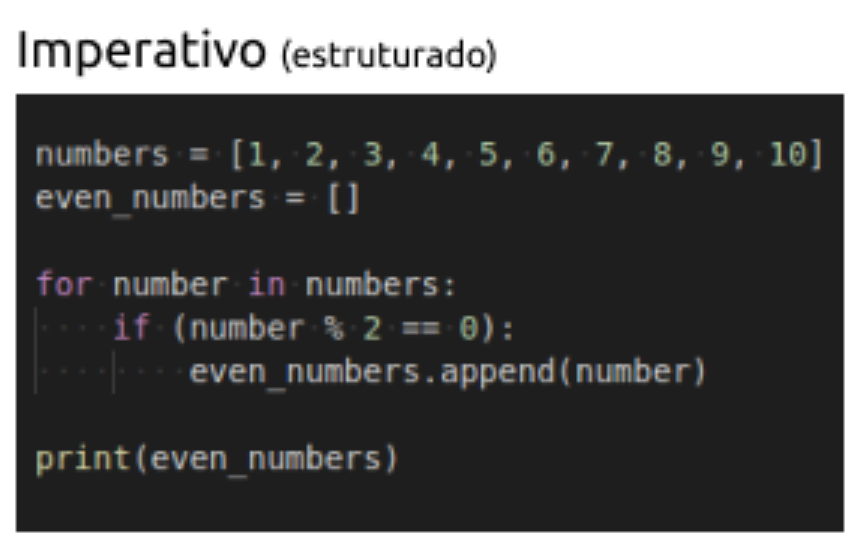
\includegraphics[width=0.6\textwidth]{imperativo.png}
  \caption{Paradigma Imperativo}
\end{figure}
\end{frame}
\begin{frame}{Paradigma Procedural}
O paradigma procedural é uma extensão do paradigma imperativo, com foco em:
\begin{itemize}
  \item Organização do código em \textbf{procedimentos ou funções};
  \item Reutilização de código;
  \item Redução da complexidade por decomposição.
\end{itemize}
\begin{figure}
  \centering
  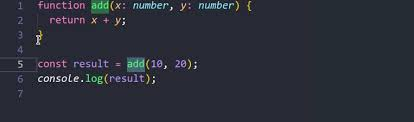
\includegraphics[width=0.8\textwidth]{procedural.jpeg}
  \caption{Paradigma Procedural}
\end{figure}
\textbf{Características principais:}
\begin{itemize}
  \item Separação entre dados e procedimentos;
  \item Estrutura modular.
\end{itemize}

\textbf{Exemplos:} C, Pascal.
\end{frame}

\begin{frame}{Paradigma Procedural}
O paradigma procedural também é muito utilizado nos hooks do Wordpress
\begin{figure}
  \centering
  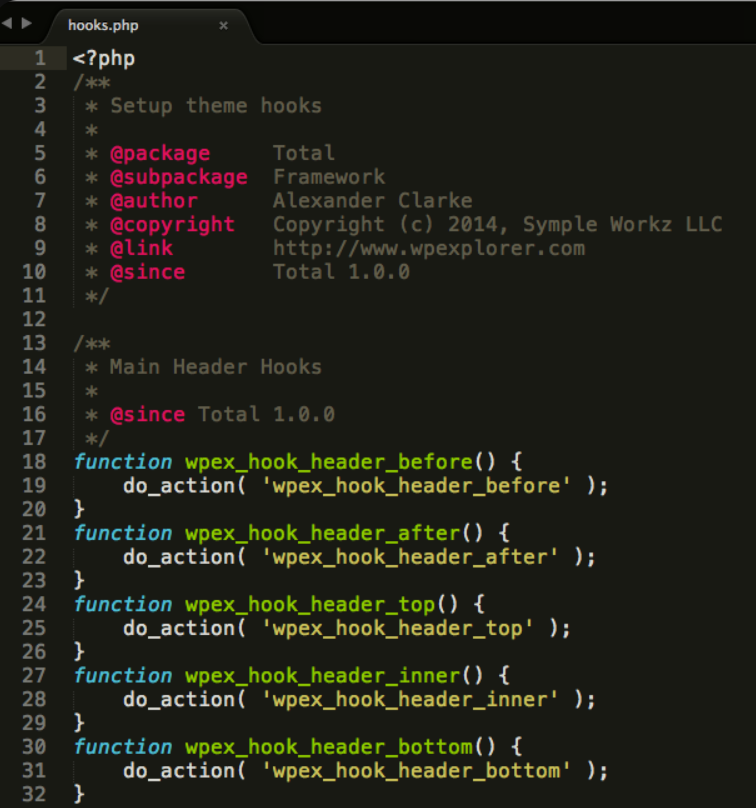
\includegraphics[width=0.5\textwidth]{wordpress.png}
  \caption{Hooks do wordpress}
\end{figure}

\end{frame}

\begin{frame}{Paradigma Orientado a Objetos}
O paradigma orientado a objetos (POO) organiza o software em  \textbf{classes}, que são moldes para os \textbf{objetos}, entidades do mundo real.\begin{figure}
\centering
\begin{minipage}{0.45\textwidth}
  \centering
  
\includegraphics[width=\textwidth]{classe_ovo.jpeg}
  \caption{Classe}
\end{minipage}
\hfill
\begin{minipage}{0.45\textwidth}
  \centering
  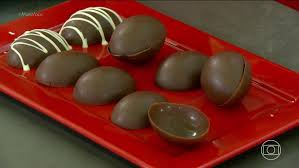
\includegraphics[width=\textwidth]{objeto_ovo.jpeg}
  \caption{Objeto}
\end{minipage}
\end{figure}


\end{frame}
\begin{frame}{Paradigma Orientado a Objetos}

\begin{figure}
  \centering
  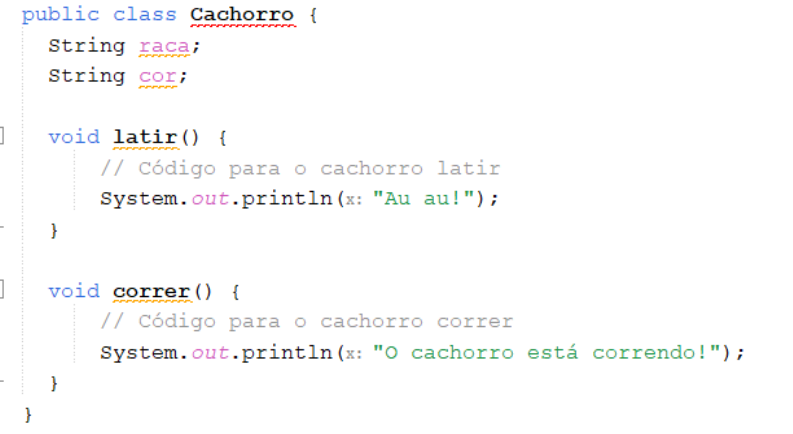
\includegraphics[width=0.7\textwidth]{poo3.png}
  \caption{Paradigma Orientado a Objetos}
\end{figure}


\end{frame}
\begin{frame}{Paradigma Orientado a Objetos}
\begin{figure}
  \centering
  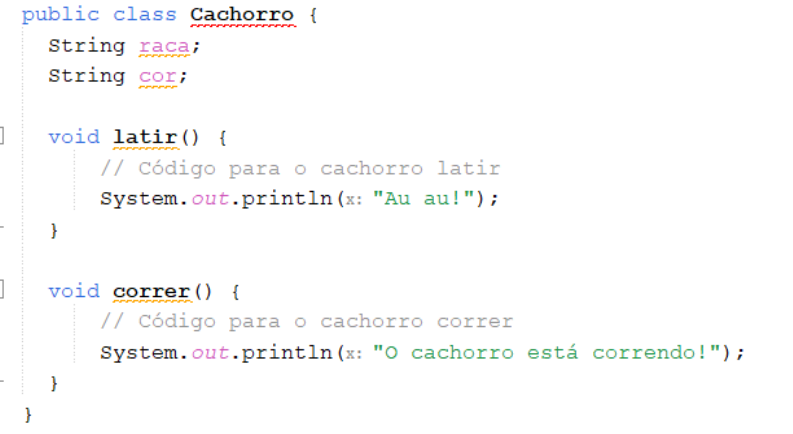
\includegraphics[width=0.7\textwidth]{poo3.png}
  \caption{Paradigma Orientado a Objetos}
\end{figure}
\textbf{Conceitos fundamentais:}
\begin{itemize}
  \item Classes e objetos;
  \item Encapsulamento;
  \item Herança;
  \item Polimorfismo.
\end{itemize}

\end{frame}
\begin{frame}{Paradigma Orientado a Objetos}


A POO favorece:
\begin{itemize}
  \item Manutenibilidade;
  \item Reuso de código;
  \item Modelagem mais próxima da realidade.
\end{itemize}

\begin{figure}
  \centering
  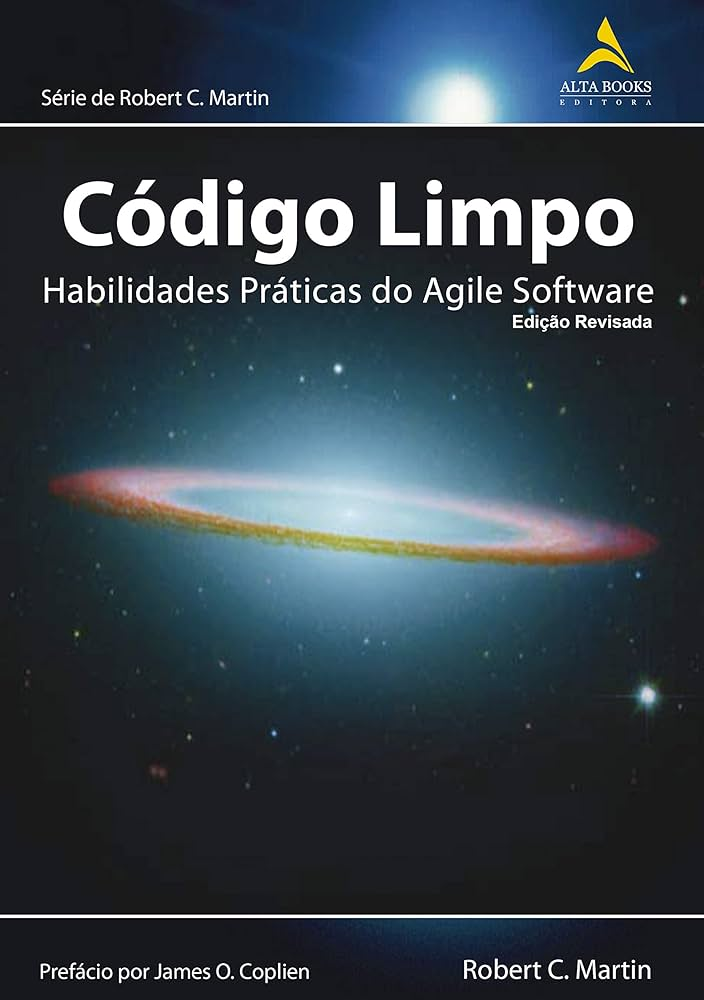
\includegraphics[width=0.3\textwidth]{clean_code.jpg}
  \caption{Clean Code}
\end{figure}

\end{frame}

\begin{frame}{Paradigma Funcional — Conceitos}
O paradigma funcional baseia-se em princípios da \textbf{matemática funcional}.

\begin{itemize}
  \item Programas são construídos a partir de \textbf{funções};
  \item Evita estados mutáveis e efeitos colaterais;
  \item Ênfase em \textbf{imutabilidade} dos dados;
  \item Uso de funções puras e recursão.
\end{itemize}
Esse paradigma favorece código previsível e mais fácil de testar.
\end{frame}
\begin{frame}{Paradigma Funcional — Características}
\begin{itemize}
  \item Funções como cidadãos de primeira classe;
  \item Alto nível de abstração;
  \item Facilita paralelismo e concorrência.
\end{itemize}

\textbf{Linguagens associadas:}
\begin{itemize}
  \item Haskell;
  \item Lisp;
  \item Scala;
  \item Uso parcial em Java, Python e JavaScript.
\end{itemize}
\end{frame}
\begin{frame}[fragile]{Exemplo — JavaScript no Paradigma Funcional}
No paradigma funcional, evita-se modificar estados e utiliza-se
funções puras e funções de alta ordem.

\begin{verbatim}
const temperaturas = [28, 30, 26, 32];

// Função pura
const celsiusParaFahrenheit = c =>
  (c * 9/5) + 32;

// Funções de alta ordem
const fahrenheit = temperaturas
  .map(celsiusParaFahrenheit)
  .filter(t => t > 86);

console.log(fahrenheit);
\end{verbatim}

\small
Exemplo de uso de imutabilidade, \texttt{map} e \texttt{filter}.
\end{frame}

\begin{frame}{Paradigma Lógico — Conceitos}
No paradigma lógico, o programa é definido por:
\begin{itemize}
  \item \textbf{Fatos};
  \item \textbf{Regras};
  \item Consultas lógicas.
\end{itemize}

O programador descreve o \textbf{problema}, e o sistema encontra a solução
por meio de inferência lógica.
\end{frame}
\begin{frame}[fragile]{Exemplo — Prolog no Paradigma Lógico}
No paradigma lógico, o programa é composto por \textbf{fatos} e
\textbf{regras}, e a execução ocorre por meio de \textbf{consultas}.

\begin{verbatim}
% Fatos
pai(joao, maria).
pai(joao, jose).
mae(ana, maria).
mae(ana, jose).

% Regra
progenitor(X, Y) :-
    pai(X, Y);
    mae(X, Y). 

% Consulta (exemplo)
% ?- progenitor(joao, maria).
\end{verbatim}

\small
O sistema utiliza inferência lógica para responder às consultas.
\end{frame}

\begin{frame}{Paradigma Lógico — Características}
\begin{itemize}
  \item Baseado em lógica de predicados;
  \item Separação entre conhecimento e controle;
  \item Uso de mecanismos de inferência automática.
\end{itemize}

\textbf{Linguagem principal:}
\begin{itemize}
  \item Prolog.
\end{itemize}

É muito utilizado em sistemas especialistas e inteligência artificial.
\end{frame}
\begin{frame}{Paradigma Declarativo — Conceitos}
No paradigma declarativo, o foco está em \textbf{o que deve ser feito},
não em \textbf{como fazer}.

\begin{itemize}
  \item O programador descreve o resultado desejado;
  \item A execução fica a cargo do sistema;
  \item Menor controle explícito do fluxo.
\end{itemize}
\end{frame}

\begin{frame}{Paradigma Declarativo — Exemplos}
\begin{itemize}
  \item SQL — consultas a bancos de dados;
  \item HTML — descrição de estrutura de páginas;
  \item Prolog — lógica declarativa.
\end{itemize}

Esse paradigma é comum em:
\begin{itemize}
  \item Bancos de dados;
  \item Linguagens de marcação;
  \item Sistemas baseados em regras.
\end{itemize}
\end{frame}





\end{document}
